\documentclass{beamer}
\usepackage{tkz-graph}
\usetikzlibrary{shapes}

%===============BEGIN GLOBAL BEAMER OPTIONS=====================

%THIS CHANGES THE BACKGROUND COLOUR OF BOXES, AND ROUNDS OFF THEIR EDGES
%\setbeamercolor{block title}{bg=yellow!50}
%\setbeamercolor{block body}{}
%\setbeamertemplate{blocks}[default]

%THIS REMOVES NAVIGATION BAR ON THE BOTTOM
\setbeamertemplate{navigation symbols}{}


%%THIS ADDS FRAME NUMBERS TO THE Right (x/y)
%\newcommand*\oldmacro{}
%\let\oldmacro\insertshorttitle
%\renewcommand*\insertshorttitle{
 %\oldmacro\hfill
 %\insertframenumber\,/\,\inserttotalframenumber}

%+++++++++++++ MODES AND THEMES +++++++++
\mode<presentation>

\usetheme{Madrid}

\usecolortheme{whale}
%\usecolortheme{crane}
%\usecolortheme{default}
%\usecolortheme{albatross}
%\usecolortheme{beetle} 
%\usecolortheme{dove} 
%\usecolortheme{fly} 
%\usecolortheme{seagull}
%\usecolortheme{rose}
%\usecolortheme{orchid}
%\usecolortheme{seahorse}



%\useoutertheme{split}
%\useoutertheme{shadow}

% USE TO CREATE PRINTER FRIENDLY HANDOUT VERSION, TOGETHER WITH [HANDOUT]
%ALSO USE ALTERNATE FIRST SLIDE
%\usecolortheme{dove}

%THIS CHANGES THE DEFAULT TRANSPARENCY GRADE FOR UNCOVERING COMMANDS
%\setbeamercovered{transparent=30}

%\beamertemplateshadingbackground{yellow!70}{black!20}

%====================================

\title[]{A common generalization of Hall's theorem and Vizing's edge-coloring theorem}
\author[landon rabern]{{\large landon rabern}}
\institute[]{~~\\~~\\
LBD Data\\
\bigskip
\bigskip
\bigskip
Miami University Colloquium\\
November 6, 2014}
\date{}

\theoremstyle{plain}
\newtheorem{thm}{Theorem}
\newtheorem{prop}[thm]{Proposition}
\newtheorem{lem}[thm]{Lemma}
\newtheorem{cor}[thm]{Corollary}

\newtheorem*{ChronicleUpdate}{\bf {Chronicle update}}
\newtheorem*{EquivalentGame}{\bf {Equivalent game}}
\newtheorem*{FixerMove}{\bf {Fixer's turn}}
\newtheorem*{BreakerMove}{\bf {Breaker's turn}}
\newtheorem*{OreBrooks}{Theorem}
\newtheorem*{PlayerMove}{Player's Move}
\newtheorem*{DealerMove}{Dealer's Move}
\newtheorem*{NecessaryCondition}{Necessary Condition}
\newtheorem*{Vizing}{Vizing's theorem}
\newtheorem*{WinningCondition}{Winning Condition}
\newtheorem*{WinningCondition2}{Winning Condition}
\newtheorem*{Winning}{Winning}
\newtheorem*{Spectrum}{Theorem}
\newtheorem*{OreBrooksKK}{Theorem}
\newtheorem*{krs1}{Theorem}
\newtheorem*{krs2}{Theorem}
\newtheorem*{BrooksTheorem}{Theorem}
\newtheorem*{MozhansLemma}{Lemma}
\newtheorem*{conjecture}{Conjecture}
\newtheorem*{PartyGame}{A prison problem}
\newtheorem{claim}{Claim}
\theoremstyle{definition}
\newtheorem{defn}{Definition}
\newtheorem*{Def}{Definition}
\newtheorem*{Degree}{Degree}
\newtheorem*{Superabundance}{Superabundance}
\theoremstyle{remark}
\newtheorem*{remark}{Remark}
\newtheorem*{goal}{Goal}
\newtheorem*{question}{Question}
\newtheorem*{observation}{Observation}

\newcommand{\fancy}[1]{\mathcal{#1}}
\newcommand{\C}[1]{\fancy{C}_{#1}}
\newcommand{\IN}{\mathbb{N}}
\newcommand{\IR}{\mathbb{R}}

\newcommand{\inj}{\hookrightarrow}
\newcommand{\surj}{\twoheadrightarrow}

\newcommand{\set}[1]{\left\{ #1 \right\}}
\newcommand{\setb}[3]{\left\{ #1 \in #2 \mid #3 \right\}}
\newcommand{\setbs}[2]{\left\{ #1 \mid #2 \right\}}
\newcommand{\card}[1]{\left|#1\right|}
\newcommand{\size}[1]{\left\Vert#1\right\Vert}
\newcommand{\ceil}[1]{\left\lceil#1\right\rceil}
\newcommand{\floor}[1]{\left\lfloor#1\right\rfloor}
\newcommand{\func}[3]{#1\colon #2 \rightarrow #3}
\newcommand{\funcinj}[3]{#1\colon #2 \inj #3}
\newcommand{\funcsurj}[3]{#1\colon #2 \surj #3}
\newcommand{\irange}[1]{\left[#1\right]}
\newcommand{\join}[2]{#1 \mbox{\hspace{2 pt}$\ast$\hspace{2 pt}} #2}
\newcommand{\djunion}[2]{#1 \mbox{\hspace{2 pt}$+$\hspace{2 pt}} #2}
\newcommand{\parens}[1]{\left( #1 \right)}

\newcommand{\DefinedAs}{\mathrel{\mathop:}=}

%\AtBeginSubsection
%{
%  \begin{frame}<beamer>{Outline}
%    \tableofcontents[currentsection,currentsubsection]
%  \end{frame}
%}

%\AtBeginSection
%{
%  \begin{frame}<beamer>{Outline}
%    \tableofcontents[currentsection,currentsubsection]
%  \end{frame}
%}

\newcommand{\1}{\item<1-> }
\newcommand{\2}{\item<2-> }
\newcommand{\3}{\item<3-> }
\newcommand{\4}{\item<4-> }
\newcommand{\5}{\item<5-> }
\newcommand{\6}{\item<6-> }
\newcommand{\7}{\item<7-> }
\newcommand{\8}{\item<8-> }
\newcommand{\9}{\item<9-> }
\newcommand{\ten}{\item<10-> }
\newcommand{\ele}{\item<11-> }
\newcommand{\twe}{\item<12-> }
\newcommand{\thi}{\item<13-> }
\newcommand{\fou}{\item<14-> }
\newcommand{\fif}{\item<15-> }
\newcommand{\six}{\item<16-> }
\newcommand{\sev}{\item<17-> }
\newcommand{\eig}{\item<18-> }

\newenvironment{dbluenv}{\color[rgb]{.2,.2,.6}}{\normalcolor}
\newcommand<>{\dblue}[1]{\begin{dbluenv}#1\end{dbluenv}}
\newcommand{\bhead}[1]{\textbf{\dblue{#1}}}
\newcommand{\pot}{\operatorname{Pot}}

\newenvironment{whiteenv}{\color[rgb]{1,1,1}}{\normalcolor}
\newcommand<>{\white}[1]{\begin{whiteenv}#1\end{whiteenv}}
\newenvironment{redenv}{\color[rgb]{.9,0,0}}{\normalcolor}
\newcommand<>{\red}[1]{\begin{redenv}#1\end{redenv}}
\newenvironment{purenv}{\color[rgb]{.8,0,.9}}{\normalcolor}
\newcommand<>{\purple}[1]{\begin{purenv}#1\end{purenv}}
\newenvironment{greenv}{\color[rgb]{0,.8,0}}{\normalcolor}
\newcommand<>{\green}[1]{\begin{greenv}#1\end{greenv}}
\newenvironment{bluenv}{\color[rgb]{0,0,.8}}{\normalcolor}
\newcommand<>{\blue}[1]{\begin{bluenv}#1\end{bluenv}}
\newenvironment{broenv}{\color[rgb]{.58,.35,.2}}{\normalcolor}
\newcommand<>{\brown}[1]{\begin{broenv}#1\end{broenv}}
\newenvironment{oraenv}{\color[rgb]{1,.41,.12}}{\normalcolor}
\newcommand<>{\orange}[1]{\begin{oraenv}#1\end{oraenv}}
\newenvironment{aquenv}{\color[cmyk]{1,0,0,0}}{\normalcolor}
\newcommand<>{\aqua}[1]{\begin{aquenv}#1\end{aquenv}}
\newenvironment{blaenv}{\color[rgb]{0,0,0}}{\normalcolor}
\newcommand<>{\black}[1]{\begin{blaenv}#1\end{blaenv}}
\newenvironment{yelenv}{\color[cmyk]{0,0,1,0}}{\normalcolor}
\newcommand<>{\yellow}[1]{\begin{yelenv}#1\end{yelenv}}

\definecolor{cf9f9f9}{RGB}{249,249,249}
\setlength{\unitlength}{5in}

\begin{document}
\setbeamertemplate{caption}{\insertcaption}
\begin{frame}
\titlepage
\end{frame}

\begin{frame}{Hall's theorem}
\begin{itemize}
\1 given finite sets $A_1, A_2, \ldots, A_n$
\2 a \red{system of distinct representatives} (SDR) is a choice of $a_i \in A_i$ for all $i$ where $a_i \ne a_j$ for $i \ne j$
\3 when can we pick an SDR?
\4 if $k$ of the sets together have fewer than $k$ elements, we can't
\begin{itemize}
\5 $A_1 = \set{1,2}$, $A_2 = \set{1,2}$, $A_3 = \set{1,2}$
\end{itemize}
\6 \red{Hall's theorem: this is the only thing that can go wrong}
\[\text{SDR exists } \Leftrightarrow \card{\bigcup_{i \in I} A_i} \ge |I| \text{ for all } I \subseteq \set{1,\ldots,n}\]
\end{itemize}
\end{frame}

\begin{frame}{some card games}{the simplest variation}
\begin{itemize}
\1 Dealer vs. Player
\2 the deck has just many copies of the high spade cards
\3 Dealer makes 5 stacks of cards with no duplicates, all cards face-up
\4 Player wins if he can pick a Royal Flush, one card from each stack
\end{itemize}

\only<1>{
\begin{picture}(1,1)
\put(0.0,0.6){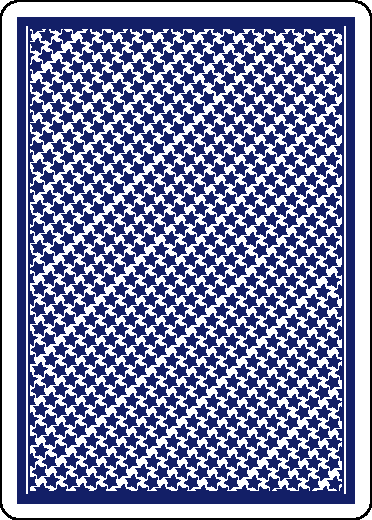
\includegraphics[width=0.15\unitlength]{cards/Back.pdf}}
\put(0.2,0.6){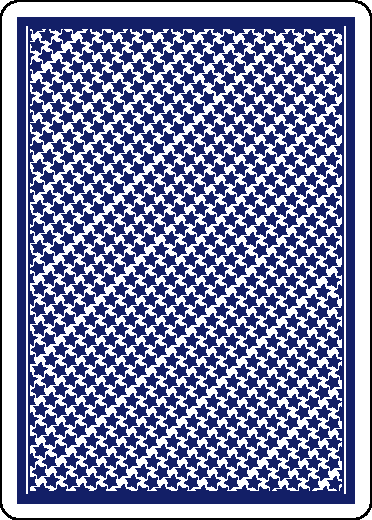
\includegraphics[width=0.15\unitlength]{cards/Back.pdf}}
\put(0.4,0.6){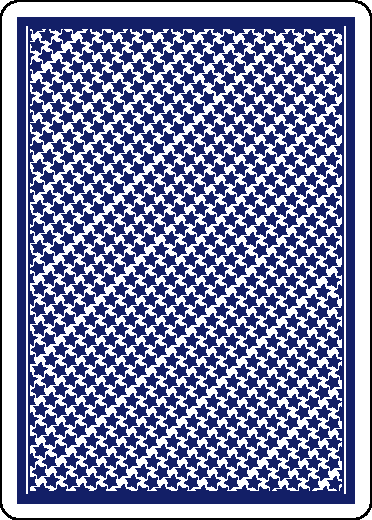
\includegraphics[width=0.15\unitlength]{cards/Back.pdf}}
\put(0.6,0.6){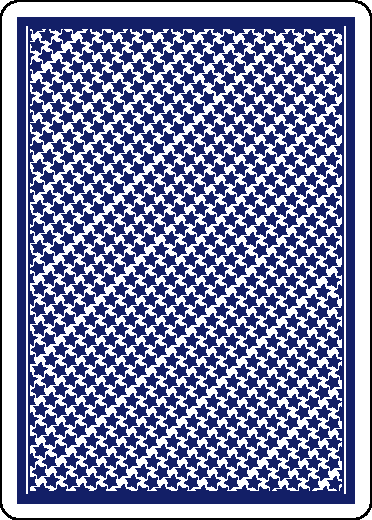
\includegraphics[width=0.15\unitlength]{cards/Back.pdf}}
\put(0.8,0.6){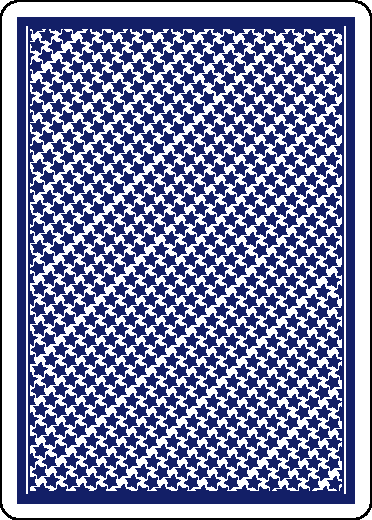
\includegraphics[width=0.15\unitlength]{cards/Back.pdf}}
\end{picture}}

\onslide<2->{
\begin{picture}(1,1)
\put(0.0,0.6){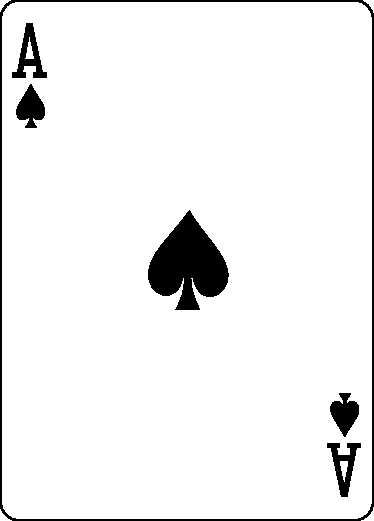
\includegraphics[width=0.15\unitlength]{cards/AS.pdf}}
\put(0.2,0.6){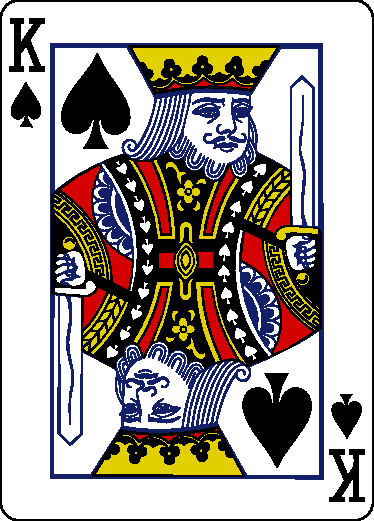
\includegraphics[width=0.15\unitlength]{cards/KS.pdf}}
\put(0.4,0.6){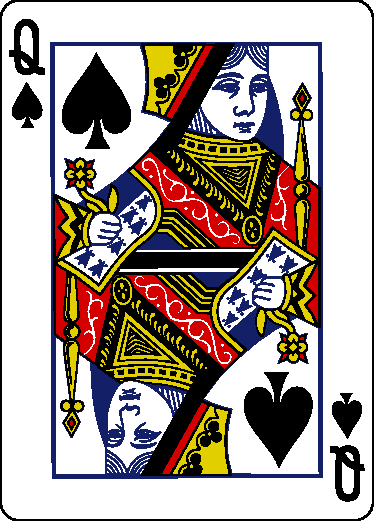
\includegraphics[width=0.15\unitlength]{cards/QS.pdf}}
\put(0.6,0.6){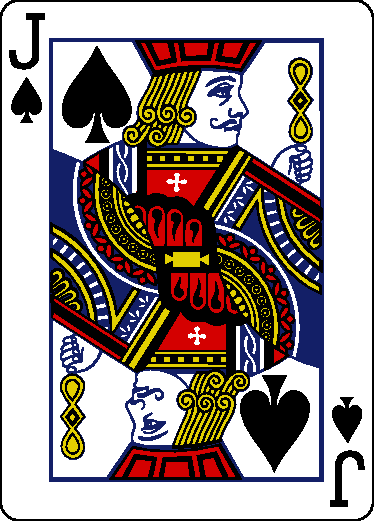
\includegraphics[width=0.15\unitlength]{cards/JS.pdf}}
\put(0.8,0.6){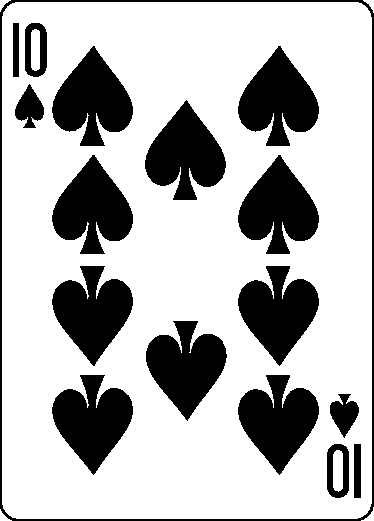
\includegraphics[width=0.15\unitlength]{cards/10S.pdf}}
\end{picture}}
\end{frame}

\begin{frame}{some card games}{example, a Player win}
\only<1>{
\begin{picture}(1,1)
\put(0.6,0.6){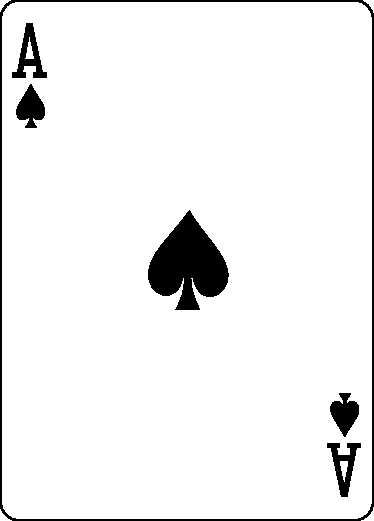
\includegraphics[width=0.15\unitlength]{cards/AS.pdf}}
\put(0.8,0.6){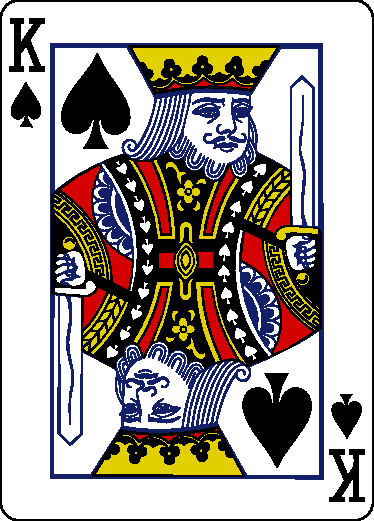
\includegraphics[width=0.15\unitlength]{cards/KS.pdf}}
\put(0.4,0.6){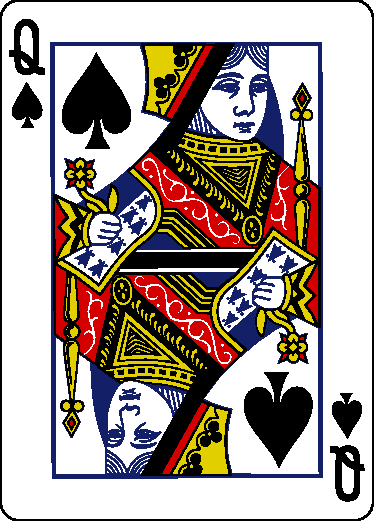
\includegraphics[width=0.15\unitlength]{cards/QS.pdf}}
\put(0.0,0.6){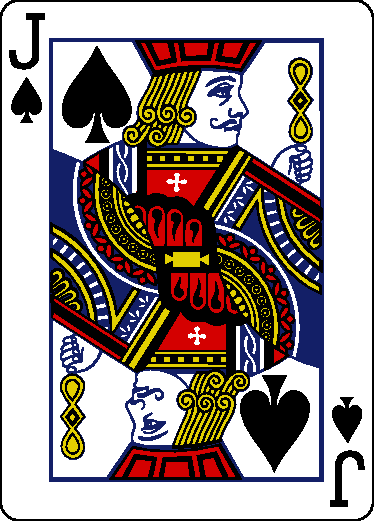
\includegraphics[width=0.15\unitlength]{cards/JS.pdf}}
\put(0.2,0.6){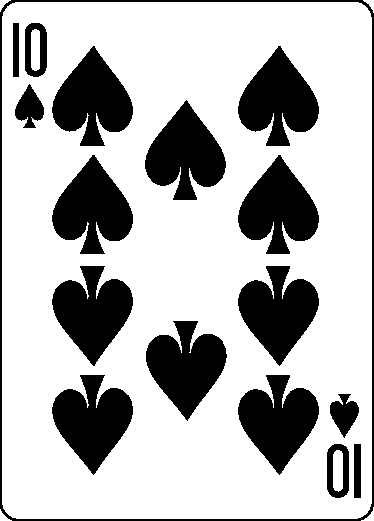
\includegraphics[width=0.15\unitlength]{cards/10S.pdf}}

\put(0.6,0.55){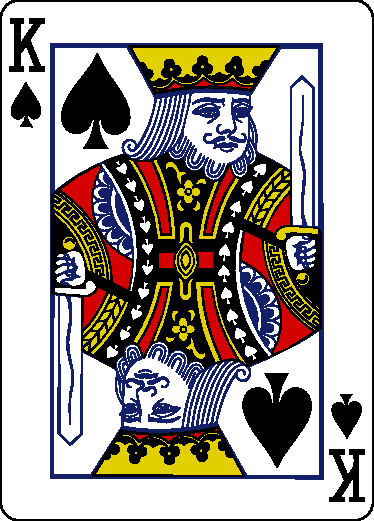
\includegraphics[width=0.15\unitlength]{cards/KS.pdf}}
\put(0.8,0.55){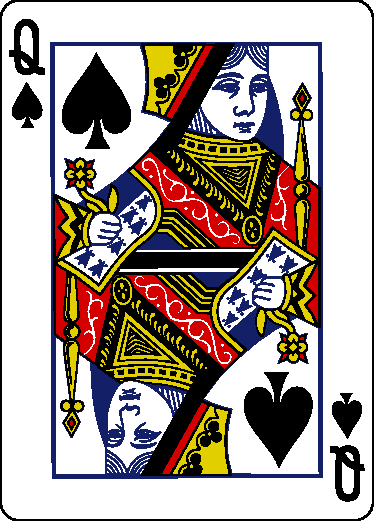
\includegraphics[width=0.15\unitlength]{cards/QS.pdf}}
\put(0.4,0.55){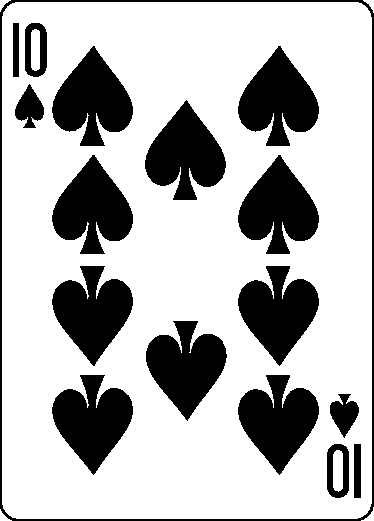
\includegraphics[width=0.15\unitlength]{cards/10S.pdf}}
\end{picture}}

\only<2>{
\begin{picture}(1,1)
\put(0.6,0.55){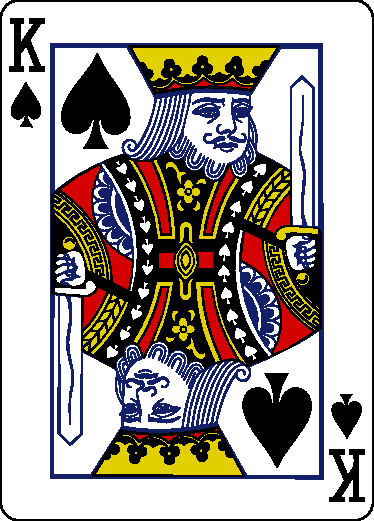
\includegraphics[width=0.15\unitlength]{cards/KS.pdf}}
\put(0.8,0.55){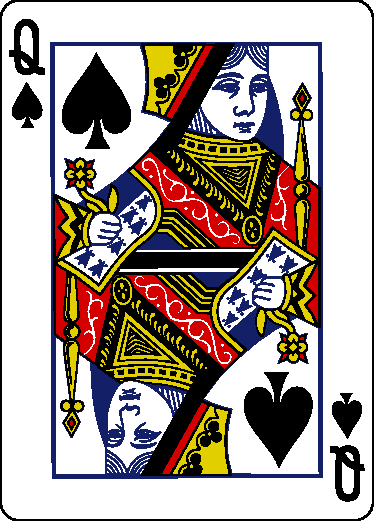
\includegraphics[width=0.15\unitlength]{cards/QS.pdf}}
\put(0.4,0.55){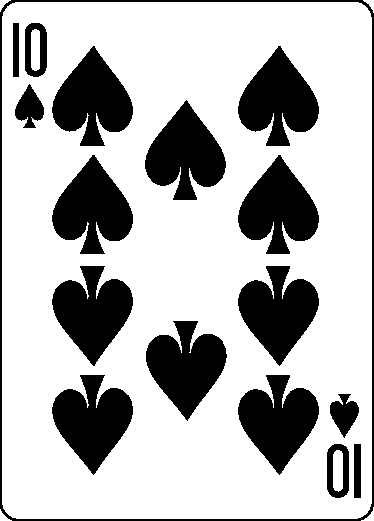
\includegraphics[width=0.15\unitlength]{cards/10S.pdf}}

\put(0.605,0.6){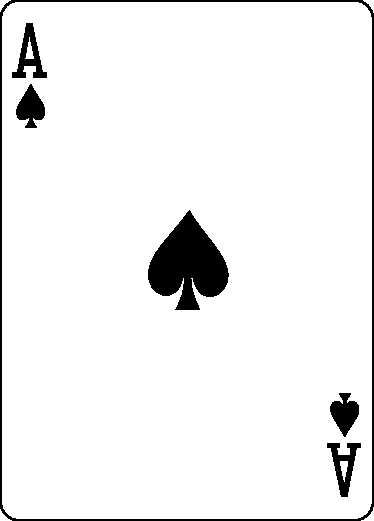
\includegraphics[width=0.17\unitlength]{cards/AS.pdf}}
\put(0.805,0.6){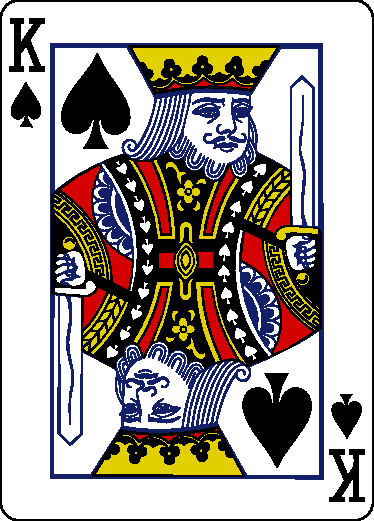
\includegraphics[width=0.17\unitlength]{cards/KS.pdf}}
\put(0.405,0.6){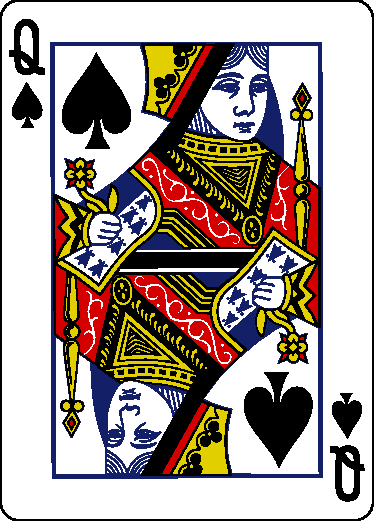
\includegraphics[width=0.17\unitlength]{cards/QS.pdf}}
\put(0.005,0.6){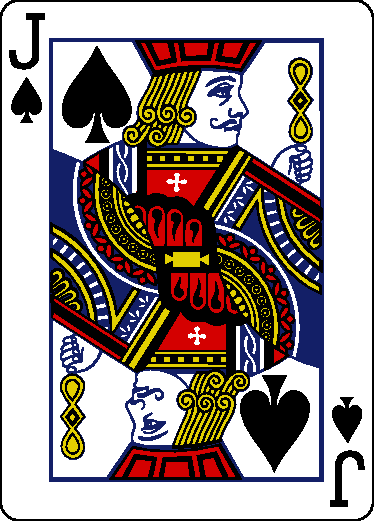
\includegraphics[width=0.17\unitlength]{cards/JS.pdf}}
\put(0.205,0.6){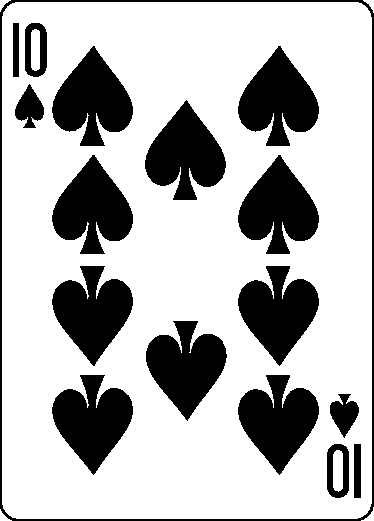
\includegraphics[width=0.17\unitlength]{cards/10S.pdf}}
\end{picture}}
\end{frame}

\begin{frame}{some card games}{example, a Dealer win}
\only<1>{
\begin{picture}(1,1)
\put(0.6,0.6){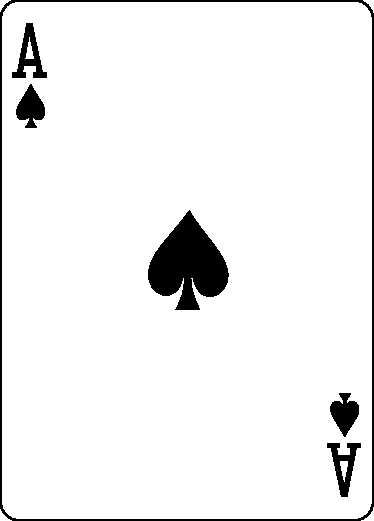
\includegraphics[width=0.15\unitlength]{cards/AS.pdf}}
\put(0.8,0.6){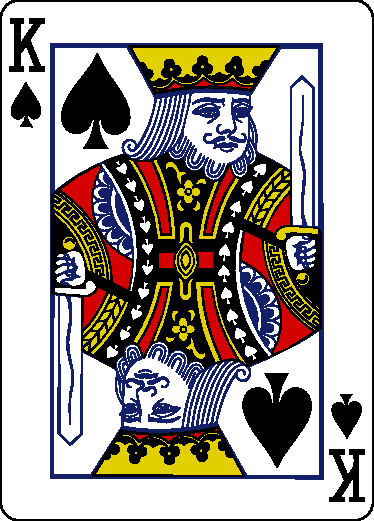
\includegraphics[width=0.15\unitlength]{cards/KS.pdf}}
\put(0.4,0.6){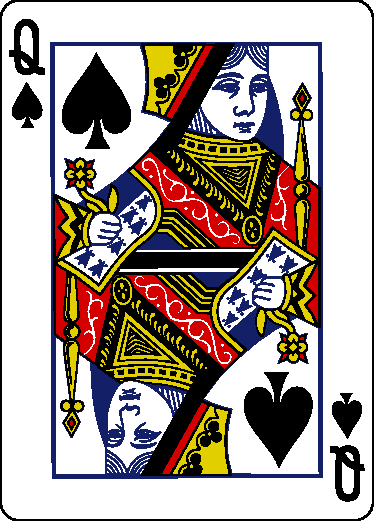
\includegraphics[width=0.15\unitlength]{cards/QS.pdf}}
\put(0.0,0.6){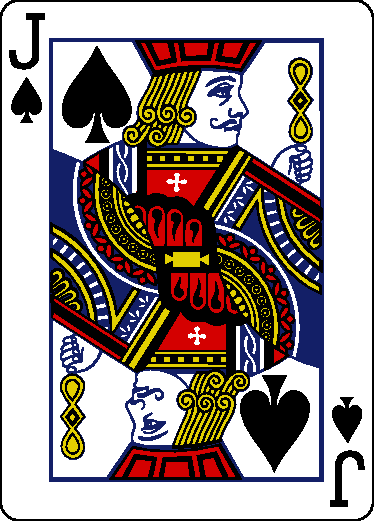
\includegraphics[width=0.15\unitlength]{cards/JS.pdf}}
\put(0.2,0.6){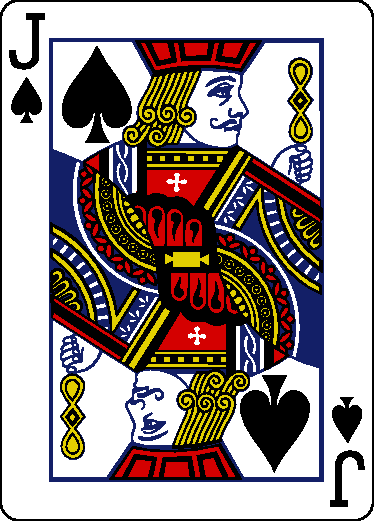
\includegraphics[width=0.15\unitlength]{cards/JS.pdf}}

\put(0.6,0.55){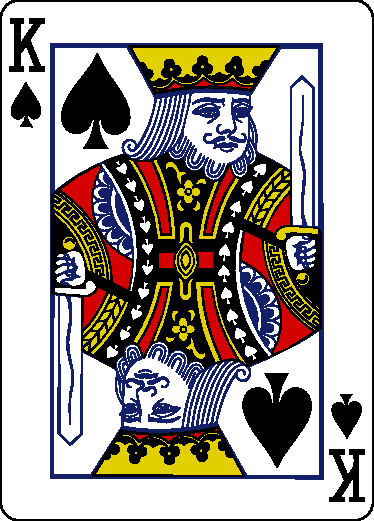
\includegraphics[width=0.15\unitlength]{cards/KS.pdf}}
\put(0.8,0.55){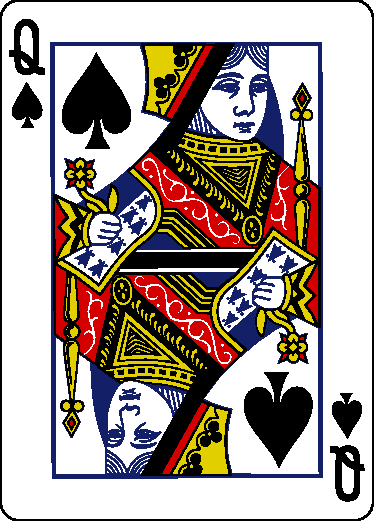
\includegraphics[width=0.15\unitlength]{cards/QS.pdf}}
\put(0.4,0.55){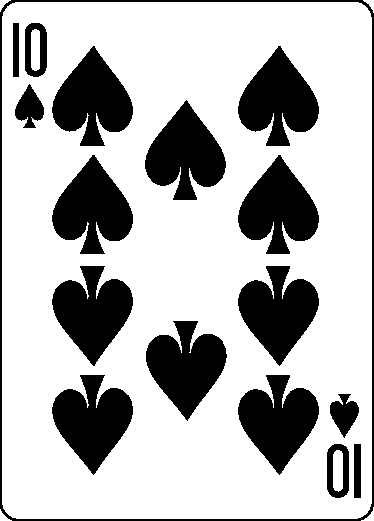
\includegraphics[width=0.15\unitlength]{cards/10S.pdf}}
\end{picture}}
\end{frame}

\begin{frame}{some card games}{winning condition}
\begin{itemize}
\1 Player cannot win if there is a set of $k$ stacks that together have fewer than $k$ different cards
\3 Hall's theorem says: \red{\textbf{Player wins otherwise}}
\end{itemize}

\onslide<2->{
\begin{picture}(1,1)
\put(0.6,0.6){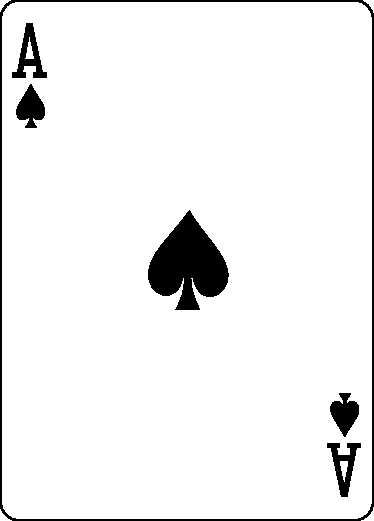
\includegraphics[width=0.15\unitlength]{cards/AS.pdf}}
\put(0.8,0.6){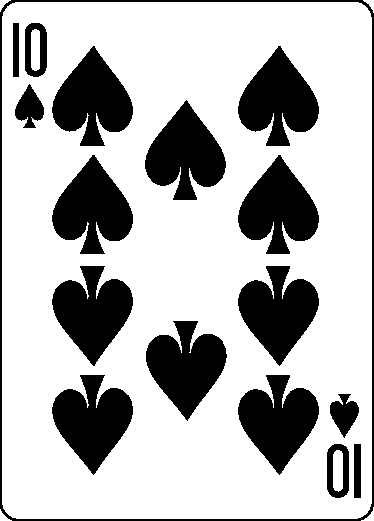
\includegraphics[width=0.15\unitlength]{cards/10S.pdf}}
\put(0.4,0.6){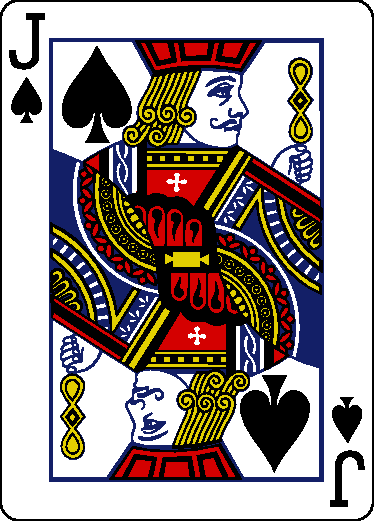
\includegraphics[width=0.15\unitlength]{cards/JS.pdf}}
\put(0.0,0.6){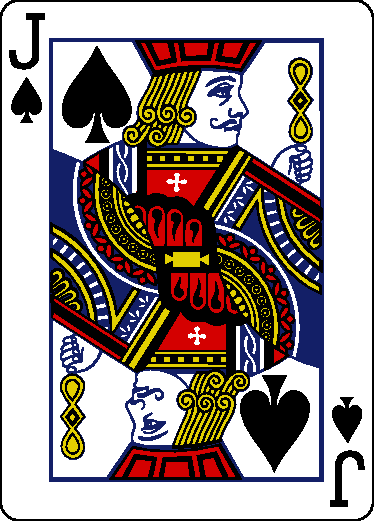
\includegraphics[width=0.15\unitlength]{cards/JS.pdf}}
\put(0.2,0.6){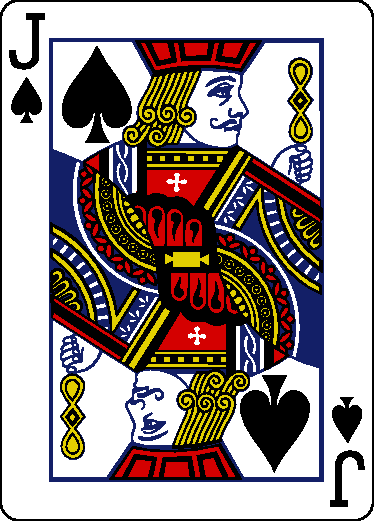
\includegraphics[width=0.15\unitlength]{cards/JS.pdf}}

\put(0.6,0.55){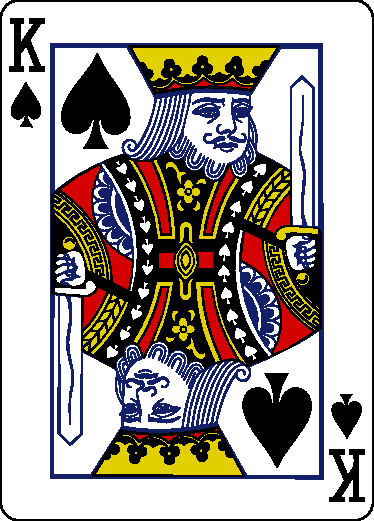
\includegraphics[width=0.15\unitlength]{cards/KS.pdf}}
\put(0.8,0.55){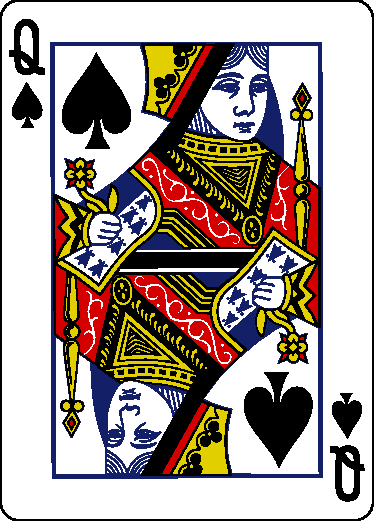
\includegraphics[width=0.15\unitlength]{cards/QS.pdf}}
\put(0.4,0.55){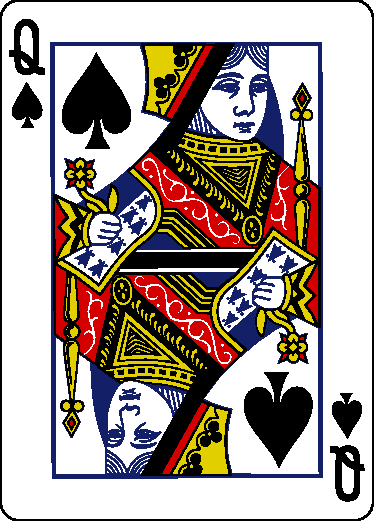
\includegraphics[width=0.15\unitlength]{cards/QS.pdf}}

\put(0.0,0.55){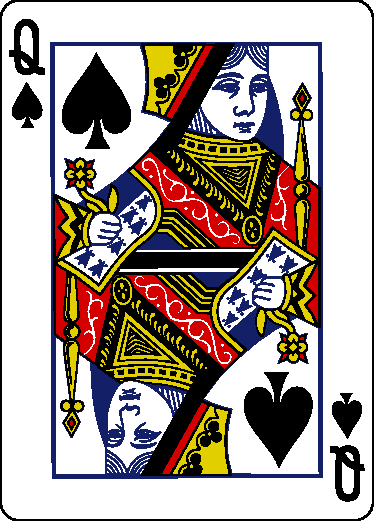
\includegraphics[width=0.15\unitlength]{cards/QS.pdf}}
\put(0.2,0.55){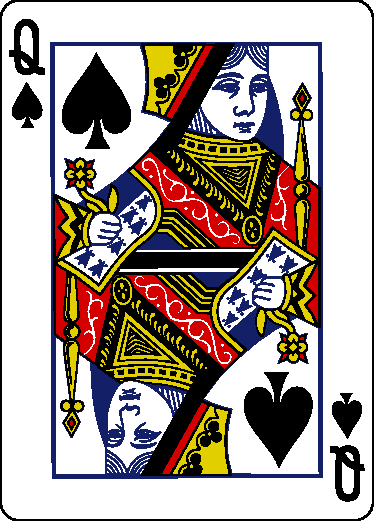
\includegraphics[width=0.15\unitlength]{cards/QS.pdf}}

\color{red}
\put(0.28, 0.69){\oval(0.6, 0.33)}
\end{picture}}
\end{frame}

\begin{frame}{some card games}{making things harder for Dealer}
\begin{itemize}
\1 this isn't a fun game, far too easy for Dealer to win
\2 to make a better game, we allow Player to modify some of the stacks
\end{itemize}

\uncover<3->{
\begin{PlayerMove}
Player can pick any card $A$ from the deck and swap it for another card $B$ in one stack (not containing $A$).
\end{PlayerMove}}

\uncover<4->{
\begin{DealerMove}
Dealer can (i) do nothing or (ii) swap $A$ and $B$ in one other stack.
\end{DealerMove}}

\uncover<5->{
\begin{Winning}
Player wins if he can pick a Royal Flush at the start of one of his turns, otherwise Dealer wins.
\end{Winning}}
\end{frame}

\begin{frame}{some card games}{example, a Player win}
\begin{itemize}
\2 Player picks a King from the deck and swaps it for a Queen in the first stack
\4 Dealer can swap a King and Queen in one of the other stacks
\6 Player wins no matter what Dealer does
\end{itemize}
\only<1>{
\begin{picture}(1,1)(0,-0.01)
\put(0.6,0.6){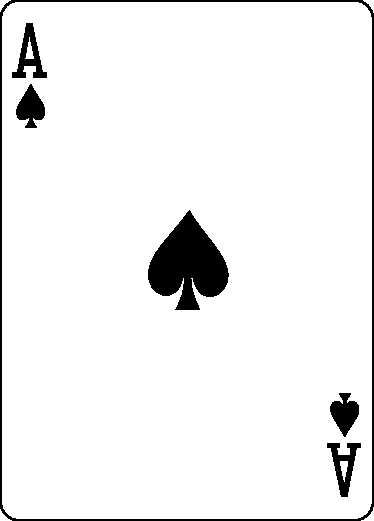
\includegraphics[width=0.15\unitlength]{cards/AS.pdf}}
\put(0.8,0.6){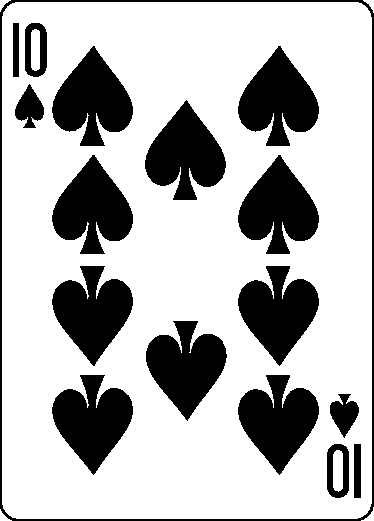
\includegraphics[width=0.15\unitlength]{cards/10S.pdf}}
\put(0.4,0.6){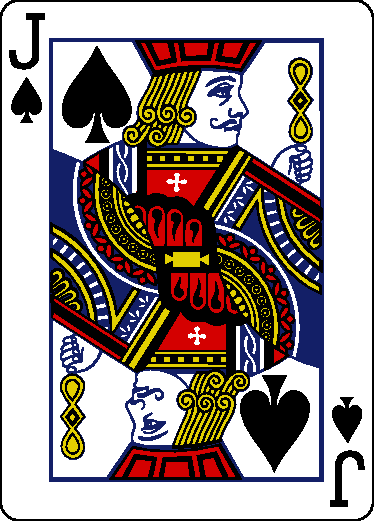
\includegraphics[width=0.15\unitlength]{cards/JS.pdf}}
\put(0.0,0.6){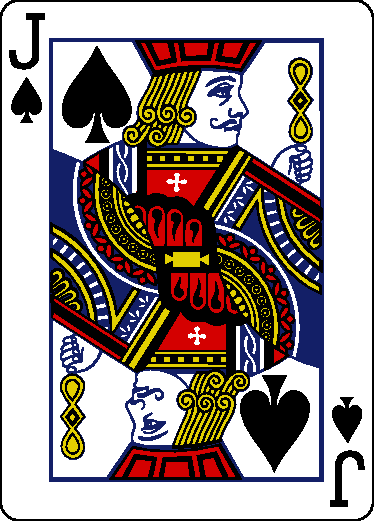
\includegraphics[width=0.15\unitlength]{cards/JS.pdf}}
\put(0.2,0.6){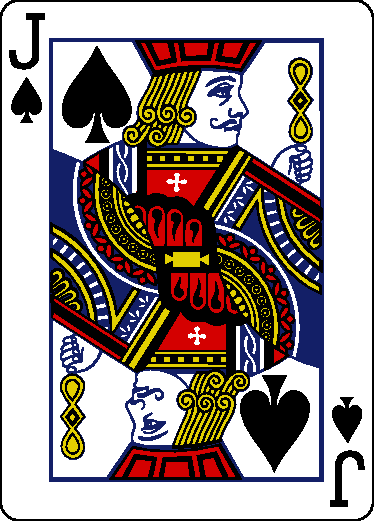
\includegraphics[width=0.15\unitlength]{cards/JS.pdf}}

\put(0.6,0.55){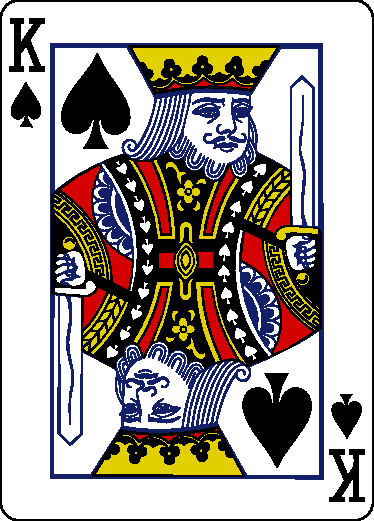
\includegraphics[width=0.15\unitlength]{cards/KS.pdf}}
\put(0.8,0.55){\includegraphics[width=0.15\unitlength]{cards/QS.pdf}}
\put(0.4,0.55){\includegraphics[width=0.15\unitlength]{cards/QS.pdf}}

\put(0.0,0.55){\includegraphics[width=0.15\unitlength]{cards/QS.pdf}}
\put(0.2,0.55){\includegraphics[width=0.15\unitlength]{cards/QS.pdf}}
\end{picture}}

\only<2>{
\begin{picture}(1,1)(0,-0.01)
\put(0.6,0.6){\includegraphics[width=0.15\unitlength]{cards/AS.pdf}}
\put(0.8,0.6){\includegraphics[width=0.15\unitlength]{cards/10S.pdf}}
\put(0.4,0.6){\includegraphics[width=0.15\unitlength]{cards/JS.pdf}}
\put(0.0,0.6){\includegraphics[width=0.15\unitlength]{cards/JS.pdf}}
\put(0.2,0.6){\includegraphics[width=0.15\unitlength]{cards/JS.pdf}}

\put(0.6,0.55){\includegraphics[width=0.15\unitlength]{cards/KS.pdf}}
\put(0.8,0.55){\includegraphics[width=0.15\unitlength]{cards/QS.pdf}}
\put(0.4,0.55){\includegraphics[width=0.15\unitlength]{cards/QS.pdf}}

\put(0.0,0.55){\includegraphics[width=0.15\unitlength]{cards/QS.pdf}}
\put(0.2,0.55){\includegraphics[width=0.15\unitlength]{cards/QS.pdf}}

\put(0.4,0.85){\includegraphics[width=0.15\unitlength]{cards/KS.pdf}}
\put(0.38,1.0){\thicklines\color{red}\vector(-1 , -1){0.22}}
\end{picture}}

\only<3>{
\begin{picture}(1,1)(0,-0.01)
\put(0.6,0.6){\includegraphics[width=0.15\unitlength]{cards/AS.pdf}}
\put(0.8,0.6){\includegraphics[width=0.15\unitlength]{cards/10S.pdf}}
\put(0.4,0.6){\includegraphics[width=0.15\unitlength]{cards/JS.pdf}}
\put(0.0,0.6){\includegraphics[width=0.15\unitlength]{cards/JS.pdf}}
\put(0.2,0.6){\includegraphics[width=0.15\unitlength]{cards/JS.pdf}}

\put(0.6,0.55){\includegraphics[width=0.15\unitlength]{cards/KS.pdf}}
\put(0.8,0.55){\includegraphics[width=0.15\unitlength]{cards/QS.pdf}}
\put(0.4,0.55){\includegraphics[width=0.15\unitlength]{cards/QS.pdf}}

\put(0.0,0.55){\includegraphics[width=0.15\unitlength]{cards/KS.pdf}}
\put(0.2,0.55){\includegraphics[width=0.15\unitlength]{cards/QS.pdf}}
\end{picture}}

\only<4>{
\begin{picture}(1,1)(0,-0.01)
\put(0.6,0.6){\includegraphics[width=0.15\unitlength]{cards/AS.pdf}}
\put(0.8,0.6){\includegraphics[width=0.15\unitlength]{cards/10S.pdf}}
\put(0.4,0.6){\includegraphics[width=0.15\unitlength]{cards/JS.pdf}}
\put(0.0,0.6){\includegraphics[width=0.15\unitlength]{cards/Back.pdf}}
\put(0.2,0.6){\includegraphics[width=0.15\unitlength]{cards/JS.pdf}}

\put(0.6,0.55){\includegraphics[width=0.15\unitlength]{cards/KS.pdf}}
\put(0.8,0.55){\includegraphics[width=0.15\unitlength]{cards/QS.pdf}}
\put(0.4,0.55){\includegraphics[width=0.15\unitlength]{cards/QS.pdf}}

\put(0.0,0.55){\includegraphics[width=0.15\unitlength]{cards/Back.pdf}}
\put(0.2,0.55){\includegraphics[width=0.15\unitlength]{cards/QS.pdf}}

\put(0.5,0.82){\includegraphics[width=0.15\unitlength]{cards/KS.pdf}}
\put(0.48,1.0){\thicklines\color{red}\vector(-1 , -1){0.17}}
\end{picture}}

\only<5>{
\begin{picture}(1,1)(0,-0.01)
\put(0.6,0.6){\includegraphics[width=0.15\unitlength]{cards/AS.pdf}}
\put(0.8,0.6){\includegraphics[width=0.15\unitlength]{cards/10S.pdf}}
\put(0.4,0.6){\includegraphics[width=0.15\unitlength]{cards/JS.pdf}}
\put(0.0,0.6){\includegraphics[width=0.15\unitlength]{cards/JS.pdf}}
\put(0.2,0.6){\includegraphics[width=0.15\unitlength]{cards/JS.pdf}}

\put(0.6,0.55){\includegraphics[width=0.15\unitlength]{cards/KS.pdf}}
\put(0.8,0.55){\includegraphics[width=0.15\unitlength]{cards/QS.pdf}}
\put(0.4,0.55){\includegraphics[width=0.15\unitlength]{cards/QS.pdf}}

\put(0.0,0.55){\includegraphics[width=0.15\unitlength]{cards/KS.pdf}}
\put(0.2,0.55){\includegraphics[width=0.15\unitlength]{cards/KS.pdf}}
\end{picture}}

\only<6>{
\begin{picture}(1,1)(0,-0.01)
\put(0.4,0.6){\includegraphics[width=0.15\unitlength]{cards/JS.pdf}}
\put(0.0,0.6){\includegraphics[width=0.15\unitlength]{cards/JS.pdf}}


\put(0.6,0.55){\includegraphics[width=0.15\unitlength]{cards/KS.pdf}}
\put(0.8,0.55){\includegraphics[width=0.15\unitlength]{cards/QS.pdf}}
\put(0.405,0.55){\includegraphics[width=0.17\unitlength]{cards/QS.pdf}}

\put(0.005,0.55){\includegraphics[width=0.17\unitlength]{cards/KS.pdf}}
\put(0.2,0.55){\includegraphics[width=0.15\unitlength]{cards/KS.pdf}}
\put(0.205,0.6){\includegraphics[width=0.17\unitlength]{cards/JS.pdf}}
\put(0.605,0.6){\includegraphics[width=0.17\unitlength]{cards/AS.pdf}}
\put(0.805,0.6){\includegraphics[width=0.17\unitlength]{cards/10S.pdf}}
\end{picture}}
\end{frame}

\begin{frame}{some card games}{example, a Dealer win}
\only<1>{
\begin{picture}(1,1)
\put(0.6,0.5){\includegraphics[width=0.15\unitlength]{cards/AS.pdf}}
\put(0.8,0.5){\includegraphics[width=0.15\unitlength]{cards/KS.pdf}}
\put(0.4,0.5){\includegraphics[width=0.15\unitlength]{cards/QS.pdf}}
\put(0.0,0.5){\includegraphics[width=0.15\unitlength]{cards/JS.pdf}}
\put(0.2,0.5){\includegraphics[width=0.15\unitlength]{cards/JS.pdf}}

\put(0.6,0.45){\includegraphics[width=0.15\unitlength]{cards/KS.pdf}}
\put(0.8,0.45){\includegraphics[width=0.15\unitlength]{cards/QS.pdf}}
\put(0.4,0.45){\includegraphics[width=0.15\unitlength]{cards/10S.pdf}}

\put(0.3,0.75){\includegraphics[width=0.15\unitlength]{cards/10S.pdf}}
\put(0.28,0.9){\thicklines\color{red}\vector(-1 , -1){0.16}}
\end{picture}}

\only<2>{
\begin{picture}(1,1)
\put(0.6,0.5){\includegraphics[width=0.15\unitlength]{cards/AS.pdf}}
\put(0.8,0.5){\includegraphics[width=0.15\unitlength]{cards/KS.pdf}}
\put(0.4,0.5){\includegraphics[width=0.15\unitlength]{cards/QS.pdf}}
\put(0.0,0.5){\includegraphics[width=0.15\unitlength]{cards/10S.pdf}}
\put(0.2,0.5){\includegraphics[width=0.15\unitlength]{cards/JS.pdf}}

\put(0.6,0.45){\includegraphics[width=0.15\unitlength]{cards/KS.pdf}}
\put(0.8,0.45){\includegraphics[width=0.15\unitlength]{cards/QS.pdf}}
\put(0.4,0.45){\includegraphics[width=0.15\unitlength]{cards/10S.pdf}}
\end{picture}}

\only<3>{
\begin{picture}(1,1)
\put(0.6,0.5){\includegraphics[width=0.15\unitlength]{cards/AS.pdf}}
\put(0.8,0.5){\includegraphics[width=0.15\unitlength]{cards/KS.pdf}}
\put(0.4,0.5){\includegraphics[width=0.15\unitlength]{cards/QS.pdf}}
\put(0.0,0.5){\includegraphics[width=0.15\unitlength]{cards/Back.pdf}}
\put(0.2,0.5){\includegraphics[width=0.15\unitlength]{cards/JS.pdf}}

\put(0.6,0.45){\includegraphics[width=0.15\unitlength]{cards/KS.pdf}}
\put(0.8,0.45){\includegraphics[width=0.15\unitlength]{cards/QS.pdf}}
\put(0.4,0.45){\includegraphics[width=0.15\unitlength]{cards/10S.pdf}}

\put(0.5,0.75){\includegraphics[width=0.15\unitlength]{cards/10S.pdf}}
\put(0.48,0.9){\thicklines\color{red}\vector(-1 , -1){0.16}}
\end{picture}}

\only<4>{
\begin{picture}(1,1)
\put(0.6,0.5){\includegraphics[width=0.15\unitlength]{cards/AS.pdf}}
\put(0.8,0.5){\includegraphics[width=0.15\unitlength]{cards/KS.pdf}}
\put(0.4,0.5){\includegraphics[width=0.15\unitlength]{cards/QS.pdf}}
\put(0.0,0.5){\includegraphics[width=0.15\unitlength]{cards/10S.pdf}}
\put(0.2,0.5){\includegraphics[width=0.15\unitlength]{cards/10S.pdf}}

\put(0.6,0.45){\includegraphics[width=0.15\unitlength]{cards/KS.pdf}}
\put(0.8,0.45){\includegraphics[width=0.15\unitlength]{cards/QS.pdf}}
\put(0.4,0.45){\includegraphics[width=0.15\unitlength]{cards/10S.pdf}}
\end{picture}}
\end{frame}

\begin{frame}{some card games}{what was the difference?}
\setlength{\unitlength}{3.5in}
\begin{itemize}
\2 in the top game, Dealer can prevent Player from increasing the number of different cards in the first two stacks
\3 in the bottom game, Dealer cannot prevent prevent Player from increasing the number of different cards in the first three stacks
\end{itemize}

\onslide<1->{
\begin{picture}(1,1)(-0.1,0.05)
\put(0.6,0.8){\includegraphics[width=0.15\unitlength]{cards/AS.pdf}}
\put(0.8,0.8){\includegraphics[width=0.15\unitlength]{cards/KS.pdf}}
\put(0.4,0.8){\includegraphics[width=0.15\unitlength]{cards/QS.pdf}}
\put(0.0,0.8){\includegraphics[width=0.15\unitlength]{cards/JS.pdf}}
\put(0.2,0.8){\includegraphics[width=0.15\unitlength]{cards/JS.pdf}}

\put(0.6,0.75){\includegraphics[width=0.15\unitlength]{cards/KS.pdf}}
\put(0.8,0.75){\includegraphics[width=0.15\unitlength]{cards/QS.pdf}}
\put(0.4,0.75){\includegraphics[width=0.15\unitlength]{cards/10S.pdf}}

\put(0.6,0.5){\includegraphics[width=0.15\unitlength]{cards/AS.pdf}}
\put(0.8,0.5){\includegraphics[width=0.15\unitlength]{cards/10S.pdf}}
\put(0.4,0.5){\includegraphics[width=0.15\unitlength]{cards/JS.pdf}}
\put(0.0,0.5){\includegraphics[width=0.15\unitlength]{cards/JS.pdf}}
\put(0.2,0.5){\includegraphics[width=0.15\unitlength]{cards/JS.pdf}}

\put(0.6,0.45){\includegraphics[width=0.15\unitlength]{cards/KS.pdf}}
\put(0.8,0.45){\includegraphics[width=0.15\unitlength]{cards/QS.pdf}}
\put(0.4,0.45){\includegraphics[width=0.15\unitlength]{cards/QS.pdf}}

\put(0.0,0.45){\includegraphics[width=0.15\unitlength]{cards/QS.pdf}}
\put(0.2,0.45){\includegraphics[width=0.15\unitlength]{cards/QS.pdf}}
\end{picture}}
\end{frame}

\begin{frame}{some card games}{necessary condition}
\begin{itemize}
\1 if the same card appears on three stacks, Player can force the addition of a new card to these stacks
\2 it is not hard to show that this is essentially all Player can do
\3 this suggests a necessary condition
\end{itemize}

\uncover<4->{
\begin{Degree}
The \emph{degree} of a card $C$ in a set of stacks $S$ is the number of times $C$ appears in $S$.  We write $d_S(C)$ for this quantity.
\end{Degree}}

\uncover<5->{
\begin{NecessaryCondition}
If Player can win, then for every set of stacks $S$ we must have 
\[\sum_{C \in \bigcup S} \ceil{\frac{d_S(C)}{2}} \ge |S|.\]
\end{NecessaryCondition}}
\end{frame}

\begin{frame}{some card games}{intuition}
\uncover<1->{
\begin{Degree}
The \emph{degree} of a card $C$ in a set of stacks $S$ is the number of times $C$ appears in $S$.  We write $d_S(C)$ for this quantity.
\end{Degree}}

\uncover<1->{
\begin{NecessaryCondition}
If Player can win, then for every set of stacks $S$ we must have 
\[\sum_{C \in \bigcup S} \ceil{\frac{d_S(C)}{2}} \ge |S|.\]
\end{NecessaryCondition}}

\begin{itemize}
\1 in Hall's theorem, each $C$ is `worth' $1$ in $\displaystyle\sum_{C \in \bigcup S} 1 = \card{\bigcup S} \ge |S|$
\2 Player can turn $2t+1$ of the same card into $t + 1$ different cards, so $C$ is `worth' $\ceil{\frac{d_S(C)}{2}}$
\end{itemize}
\end{frame}

\begin{frame}{some card games}{Dealer's strategy}
\begin{itemize}
\1 given a set of stacks $S$ with $\displaystyle\sum_{C \in \bigcup S} \ceil{\frac{d_S(C)}{2}} < |S|$
\2 Dealer's strategy: \red{maintain this invariant}
\begin{itemize}
\3 this is good enough since then $\card{\bigcup S} \le \displaystyle\sum_{C \in \bigcup S} \ceil{\frac{d_S(C)}{2}} < |S|$ always
\4 if Player swaps $A$ in for $B$, increasing $\ceil{\frac{d_S(A)}{2}} + \ceil{\frac{d_S(B)}{2}}$, then $d_S(A)$ and $d_S(B)$ both changed from even to odd
\5 so, Dealer can swap $A$ for $B$ somewhere else, decreasing $\ceil{\frac{d_S(A)}{2}} + \ceil{\frac{d_S(B)}{2}}$
\6 Dealer has maintained $\displaystyle\sum_{C \in \bigcup S} \ceil{\frac{d_S(C)}{2}} < |S|$
\end{itemize}
\end{itemize}
\end{frame}

\begin{frame}{some card games}{winning condition}
\begin{itemize}
\1 \red{\textbf{this necessary condition is also suffcient}}
\end{itemize}
\uncover<2->{
\begin{WinningCondition}
Player can win if and only if for every set of stacks $S$ we have 
\[\sum_{C \in \bigcup S} \ceil{\frac{d_S(C)}{2}} \ge |S|.\]
\end{WinningCondition}}
\end{frame}

\begin{frame}{some card games}{proof idea}
\setlength{\unitlength}{5in}
\begin{enumerate}
\1 Player looks for a set of card types that give a system of distinct representatives of all the stacks containing them
\5 Player calls those stacks done and never plays with those card types again
\end{enumerate}

\only<1>{
\begin{picture}(1,1)(0.0, -0.11)
\put(0.6,0.5){\includegraphics[width=0.15\unitlength]{cards/AS.pdf}}
\put(0.8,0.5){\includegraphics[width=0.15\unitlength]{cards/10S.pdf}}
\put(0.4,0.5){\includegraphics[width=0.15\unitlength]{cards/JS.pdf}}
\put(0.0,0.5){\includegraphics[width=0.15\unitlength]{cards/JS.pdf}}
\put(0.2,0.5){\includegraphics[width=0.15\unitlength]{cards/JS.pdf}}

\put(0.6,0.45){\includegraphics[width=0.15\unitlength]{cards/10S.pdf}}
\put(0.8,0.45){\includegraphics[width=0.15\unitlength]{cards/QS.pdf}}
\put(0.4,0.45){\includegraphics[width=0.15\unitlength]{cards/QS.pdf}}

\put(0.0,0.45){\includegraphics[width=0.15\unitlength]{cards/QS.pdf}}
\put(0.2,0.45){\includegraphics[width=0.15\unitlength]{cards/QS.pdf}}
\end{picture}}
\only<2>{
\begin{picture}(1,1)(0.0, -0.11)
\put(0.6,0.5){\includegraphics[width=0.15\unitlength]{cards/AS.pdf}}
\put(0.805,0.5){\includegraphics[width=0.17\unitlength]{cards/10S.pdf}}
\put(0.4,0.5){\includegraphics[width=0.15\unitlength]{cards/JS.pdf}}
\put(0.0,0.5){\includegraphics[width=0.15\unitlength]{cards/JS.pdf}}
\put(0.2,0.5){\includegraphics[width=0.15\unitlength]{cards/JS.pdf}}

\put(0.605,0.45){\includegraphics[width=0.17\unitlength]{cards/10S.pdf}}
\put(0.8,0.45){\includegraphics[width=0.15\unitlength]{cards/QS.pdf}}
\put(0.4,0.45){\includegraphics[width=0.15\unitlength]{cards/QS.pdf}}

\put(0.0,0.45){\includegraphics[width=0.15\unitlength]{cards/QS.pdf}}
\put(0.2,0.45){\includegraphics[width=0.15\unitlength]{cards/QS.pdf}}
\end{picture}}
\only<3>{
\begin{picture}(1,1)(0.0, -0.11)
\put(0.6,0.5){\includegraphics[width=0.15\unitlength]{cards/AS.pdf}}
\put(0.8,0.5){\includegraphics[width=0.15\unitlength]{cards/10S.pdf}}
\put(0.4,0.5){\includegraphics[width=0.15\unitlength]{cards/JS.pdf}}
\put(0.0,0.5){\includegraphics[width=0.15\unitlength]{cards/JS.pdf}}
\put(0.2,0.5){\includegraphics[width=0.15\unitlength]{cards/JS.pdf}}

\put(0.6,0.45){\includegraphics[width=0.15\unitlength]{cards/10S.pdf}}
\put(0.8,0.45){\includegraphics[width=0.15\unitlength]{cards/QS.pdf}}
\put(0.4,0.45){\includegraphics[width=0.15\unitlength]{cards/QS.pdf}}

\put(0.0,0.45){\includegraphics[width=0.15\unitlength]{cards/QS.pdf}}
\put(0.2,0.45){\includegraphics[width=0.15\unitlength]{cards/QS.pdf}}
\end{picture}}
\only<4>{
\begin{picture}(1,1)(0.0, -0.11)
\put(0.605,0.5){\includegraphics[width=0.17\unitlength]{cards/AS.pdf}}
\put(0.805,0.5){\includegraphics[width=0.17\unitlength]{cards/10S.pdf}}
\put(0.4,0.5){\includegraphics[width=0.15\unitlength]{cards/JS.pdf}}
\put(0.0,0.5){\includegraphics[width=0.15\unitlength]{cards/JS.pdf}}
\put(0.2,0.5){\includegraphics[width=0.15\unitlength]{cards/JS.pdf}}

\put(0.6,0.45){\includegraphics[width=0.15\unitlength]{cards/10S.pdf}}
\put(0.8,0.45){\includegraphics[width=0.15\unitlength]{cards/QS.pdf}}
\put(0.4,0.45){\includegraphics[width=0.15\unitlength]{cards/QS.pdf}}

\put(0.0,0.45){\includegraphics[width=0.15\unitlength]{cards/QS.pdf}}
\put(0.2,0.45){\includegraphics[width=0.15\unitlength]{cards/QS.pdf}}
\end{picture}}
\only<5>{
\begin{picture}(1,1)(0.0, -0.11)
\put(0.6,0.5){\includegraphics[width=0.15\unitlength]{cards/back.pdf}}
\put(0.8,0.5){\includegraphics[width=0.15\unitlength]{cards/back.pdf}}

\put(0.4,0.5){\includegraphics[width=0.15\unitlength]{cards/JS.pdf}}
\put(0.0,0.5){\includegraphics[width=0.15\unitlength]{cards/JS.pdf}}
\put(0.2,0.5){\includegraphics[width=0.15\unitlength]{cards/JS.pdf}}

\put(0.6,0.45){\includegraphics[width=0.15\unitlength]{cards/back.pdf}}
\put(0.8,0.45){\includegraphics[width=0.15\unitlength]{cards/back.pdf}}

\put(0.4,0.45){\includegraphics[width=0.15\unitlength]{cards/QS.pdf}}

\put(0.0,0.45){\includegraphics[width=0.15\unitlength]{cards/QS.pdf}}
\put(0.2,0.45){\includegraphics[width=0.15\unitlength]{cards/QS.pdf}}
\end{picture}}
\end{frame}

\begin{frame}{some card games}{proof idea}
\begin{enumerate}
\setcounter{enumi}{2}
\1 if no such set of card types exists, then Hall's theorem shows that there is at least one card appearing on none of the remaining stacks
\2 but then some card appears at least thrice, so Player can increase the number of card types in the stacks
\3 goto step 1
\end{enumerate}

\only<1>{
\begin{picture}(1,1)(0.0, -0.1475)
\put(0.6,0.5){\includegraphics[width=0.15\unitlength]{cards/back.pdf}}
\put(0.8,0.5){\includegraphics[width=0.15\unitlength]{cards/back.pdf}}

\put(0.4,0.5){\includegraphics[width=0.15\unitlength]{cards/JS.pdf}}
\put(0.0,0.5){\includegraphics[width=0.15\unitlength]{cards/JS.pdf}}
\put(0.2,0.5){\includegraphics[width=0.15\unitlength]{cards/JS.pdf}}

\put(0.6,0.45){\includegraphics[width=0.15\unitlength]{cards/back.pdf}}
\put(0.8,0.45){\includegraphics[width=0.15\unitlength]{cards/back.pdf}}

\put(0.4,0.45){\includegraphics[width=0.15\unitlength]{cards/QS.pdf}}

\put(0.0,0.45){\includegraphics[width=0.15\unitlength]{cards/QS.pdf}}
\put(0.2,0.45){\includegraphics[width=0.15\unitlength]{cards/QS.pdf}}
\end{picture}}
\only<2>{
\begin{picture}(1,1)(0.0, -0.1475)
\put(0.6,0.5){\includegraphics[width=0.15\unitlength]{cards/back.pdf}}
\put(0.8,0.5){\includegraphics[width=0.15\unitlength]{cards/back.pdf}}

\put(0.4,0.5){\includegraphics[width=0.15\unitlength]{cards/JS.pdf}}
\put(0.0,0.5){\includegraphics[width=0.15\unitlength]{cards/JS.pdf}}
\put(0.2,0.5){\includegraphics[width=0.15\unitlength]{cards/JS.pdf}}

\put(0.6,0.45){\includegraphics[width=0.15\unitlength]{cards/back.pdf}}
\put(0.8,0.45){\includegraphics[width=0.15\unitlength]{cards/back.pdf}}

\put(0.4,0.45){\includegraphics[width=0.15\unitlength]{cards/QS.pdf}}

\put(0.0,0.45){\includegraphics[width=0.15\unitlength]{cards/QS.pdf}}
\put(0.2,0.45){\includegraphics[width=0.15\unitlength]{cards/QS.pdf}}

\put(0.52,0.72){\includegraphics[width=0.15\unitlength]{cards/KS.pdf}}
\put(0.48,0.88){\thicklines\color{red}\vector(-2 , -1){0.35}}
\end{picture}}
\only<3>{
\begin{picture}(1,1)(0.0, -0.1475)
\put(0.6,0.5){\includegraphics[width=0.15\unitlength]{cards/back.pdf}}
\put(0.8,0.5){\includegraphics[width=0.15\unitlength]{cards/back.pdf}}

\put(0.4,0.5){\includegraphics[width=0.15\unitlength]{cards/JS.pdf}}
\put(0.0,0.5){\includegraphics[width=0.15\unitlength]{cards/JS.pdf}}
\put(0.2,0.5){\includegraphics[width=0.15\unitlength]{cards/JS.pdf}}

\put(0.6,0.45){\includegraphics[width=0.15\unitlength]{cards/back.pdf}}
\put(0.8,0.45){\includegraphics[width=0.15\unitlength]{cards/back.pdf}}

\put(0.4,0.45){\includegraphics[width=0.15\unitlength]{cards/QS.pdf}}

\put(0.0,0.45){\includegraphics[width=0.15\unitlength]{cards/KS.pdf}}
\put(0.2,0.45){\includegraphics[width=0.15\unitlength]{cards/QS.pdf}}
\end{picture}}

\only<4>{
\begin{picture}(1,1)(0.0, -0.1475)
\put(0.6,0.5){\includegraphics[width=0.15\unitlength]{cards/back.pdf}}
\put(0.8,0.5){\includegraphics[width=0.15\unitlength]{cards/back.pdf}}

\put(0.4,0.5){\includegraphics[width=0.15\unitlength]{cards/JS.pdf}}
\put(0.0,0.5){\includegraphics[width=0.15\unitlength]{cards/back.pdf}}
\put(0.2,0.5){\includegraphics[width=0.15\unitlength]{cards/JS.pdf}}

\put(0.6,0.45){\includegraphics[width=0.15\unitlength]{cards/back.pdf}}
\put(0.8,0.45){\includegraphics[width=0.15\unitlength]{cards/back.pdf}}

\put(0.4,0.45){\includegraphics[width=0.15\unitlength]{cards/QS.pdf}}

\put(0.0,0.45){\includegraphics[width=0.15\unitlength]{cards/back.pdf}}
\put(0.2,0.45){\includegraphics[width=0.15\unitlength]{cards/QS.pdf}}
\end{picture}}

\only<5>{
\begin{picture}(1,1)(0.0, -0.1475)
\put(0.6,0.5){\includegraphics[width=0.15\unitlength]{cards/back.pdf}}
\put(0.8,0.5){\includegraphics[width=0.15\unitlength]{cards/back.pdf}}

\put(0.4,0.5){\includegraphics[width=0.15\unitlength]{cards/JS.pdf}}
\put(0.0,0.5){\includegraphics[width=0.15\unitlength]{cards/back.pdf}}
\put(0.205,0.5){\includegraphics[width=0.17\unitlength]{cards/JS.pdf}}

\put(0.6,0.45){\includegraphics[width=0.15\unitlength]{cards/back.pdf}}
\put(0.8,0.45){\includegraphics[width=0.15\unitlength]{cards/back.pdf}}

\put(0.405,0.45){\includegraphics[width=0.17\unitlength]{cards/QS.pdf}}

\put(0.0,0.45){\includegraphics[width=0.15\unitlength]{cards/back.pdf}}
\put(0.2,0.45){\includegraphics[width=0.15\unitlength]{cards/QS.pdf}}
\end{picture}}

\only<6>{
\begin{picture}(1,1)(0.0, -0.1475)
\put(0.605,0.5){\includegraphics[width=0.17\unitlength]{cards/AS.pdf}}
\put(0.805,0.5){\includegraphics[width=0.17\unitlength]{cards/10S.pdf}}
\put(0.4,0.5){\includegraphics[width=0.15\unitlength]{cards/JS.pdf}}
\put(0.0,0.5){\includegraphics[width=0.15\unitlength]{cards/JS.pdf}}
\put(0.205,0.5){\includegraphics[width=0.17\unitlength]{cards/JS.pdf}}

\put(0.6,0.45){\includegraphics[width=0.15\unitlength]{cards/10S.pdf}}
\put(0.8,0.45){\includegraphics[width=0.15\unitlength]{cards/QS.pdf}}
\put(0.405,0.45){\includegraphics[width=0.17\unitlength]{cards/QS.pdf}}

\put(0.005,0.45){\includegraphics[width=0.17\unitlength]{cards/KS.pdf}}
\put(0.2,0.45){\includegraphics[width=0.15\unitlength]{cards/QS.pdf}}
\end{picture}}
\end{frame}

\begin{frame}{A generalization of Hall's theorem}{making it harder for Player}
\begin{itemize}
\1 allow Dealer to make more swaps in response to Player's move
\2 for each $t \ge 1$, the \red{$t$-game} allows Dealer to make up to $t$ swaps
\end{itemize}

\uncover<3->{
\begin{WinningCondition}
Player can win in the $t$-game if and only if for every set of stacks $S$ we have 
\[\sum_{C \in \bigcup S} \ceil{\frac{d_S(C)}{t + 1}} \ge |S|.\]
\end{WinningCondition}}
\begin{itemize}
\4 Hall's theorem is the winning condition in the $(k-1)$-game when there are $k$ total stacks:
\begin{itemize}
\5 $1 \le d_S(C) \le k$, so $\ceil{\frac{d_S(C)}{t + 1}} = 1$
\6 so, the sum equals $\card{\bigcup S}$
\7 Player's moves are useless
\end{itemize}
\end{itemize}
\end{frame}

\begin{frame}{edge coloring}{setup}
\begin{itemize}
\1 assign colors to the edges of a graph so that incident edges get different colors
\2 how few colors can we use?
\end{itemize}

\uncover<3->{
\begin{Vizing}
Any simple graph can be edge-colored using at most one more color than its maximum degree.
\end{Vizing}}
\end{frame}

\begin{frame}{edge coloring}{proof of Vizing's theorem}
\begin{itemize}
\1 proceed by induction on the number of vertices
\2 remove a vertex and edge-color the rest with one more color than its maximum degree
\end{itemize}

\begin{center}
\resizebox{2in}{!}{
\includegraphics<1>{graphs/g1}
\includegraphics<2>{graphs/g2}
\includegraphics<3>{graphs/g3}
\includegraphics<4>{graphs/g4}
\includegraphics<5>{graphs/g5}
\includegraphics<6>{graphs/g6}
\includegraphics<7>{graphs/g7}
\includegraphics<8>{graphs/g8}
}
\end{center}
\end{frame}

\begin{frame}{edge coloring}{proof of Vizing's theorem}
\begin{itemize}
\1 \textbf{\red{exchanging colors on a two-colored path is just a Player move followed by a Dealer move}}
\2 we can make any of Player's legal moves this way, so if the winning conditions are satisfied, Vizing's theorem is true
\3 each stack has at least two colors, so counting the `cards' in two ways we get for each set of stacks $S$,
\[\sum_{C \in \bigcup S} d_S(C) \ge 2|S|\]
\4 so, we have the desired winning condition
\[\sum_{C \in \bigcup S} \frac{d_S(C)}{2} \ge |S|\]
\end{itemize}
\end{frame}

\begin{frame}{summary}
\begin{itemize}
\1 we introduced a simple card game
\begin{itemize}
\2 Player can pick any card $A$ from the deck and swap it for another card $B$ in one stack (not containing $A$)
\3 Dealer can (i) do nothing or (ii) swap $A$ and $B$ in one other stack
\4 Player wins if he can pick a Royal Flush at the start of one of his turns, otherwise Dealer wins
\end{itemize}
\5 Player can win exactly when a Hall-like condition is satisfied
\6 Vizing's edge-coloring theorem is an easy corollary
\7 taking it further
\begin{itemize}
\8 most other classical edge-coloring results follow easily
\9 generalizes easily to multigraphs
\ten a more general game unifies much of edge-coloring theory
\end{itemize}
\end{itemize}
\end{frame}

\begin{frame}{the more general game}
\begin{itemize}
\1 Fixer vs. Breaker
\2 played on a multigraph $G$
\3 assign a list of colors $L(v)$ to each vertex
\4 let the \red{pot} be $\bigcup_{v \in V(G)} L(v)$
\5 Fixer wins if at the start of his turn he can construct an edge-coloring $\pi$ of $G$ where $\pi(xy) \in L(x) \cap L(y)$ for each $xy \in E(G)$
\end{itemize}
\uncover<6->{
\begin{FixerMove}
Pick $\alpha$ in the pot and $v \in V(G)$ with $\alpha \not \in L(v)$ and set $L(v)
\DefinedAs L(v) \cup \set{\alpha} - \beta$ for some $\beta
\in L(v)$.
\end{FixerMove}}

\uncover<7->{
\begin{BreakerMove}
If Fixer modified $L(v)$ by inserting $\alpha$ and removing $\beta$, then
Breaker can either do nothing or pick $w \in V(G - v)$ and modify its list by
swapping $\alpha$ for $\beta$ or $\beta$ for $\alpha$.
\end{BreakerMove}}
\end{frame}


\begin{frame}{the more general game}{necessary condition}
\uncover<1->{
\begin{Def}
For $C \subseteq \pot(L)$ and $H \subseteq G$, let $H_{L, C}$ be the
subgraph of $H$ induced on the vertices $v$ with $L(v) \cap C \ne \emptyset$. For $H \subseteq G$, put

\[\psi_L(H) = \sum_{\alpha \in \pot(L)} \floor{\frac{\card{H_{L, \alpha}}}{2}}.\]
\end{Def}}

\uncover<2->{
\begin{Superabundance}
We say that $(H, L)$ is \red{abundant} if $\psi_L(H) \ge \size{H}$ and that $(H,L)$ is \red{superabundant} if for every
$H' \subseteq H$, the pair $(H', L)$ is abundant.
\end{Superabundance}}

\uncover<3->{
\begin{NecessaryCondition}
If Fixer can win, then $(G, L)$ is superabundant.
\end{NecessaryCondition}}
\end{frame}

\begin{frame}{the more general game}{adding a chronicle}
\begin{itemize}
\1 we can get more power for Fixer and still imply edge-coloring results by modifying the game slightly
\2 we do this by adding a \red{chronicle}
\3 basically, this ensures that Breaker's moves are consistent with being embedded \emph{some} graph
\4 the \red{chronicle} $C$ is a multigraph with vertex set $V(G) \cup \set{\infty}$ that will be updated as the game progresses.  Each edge of
$C$ will be labeled with a doubleton of colors $\set{\alpha, \beta} \subseteq \pot(L)$.  At the start of the game $C$ is edgeless.
\end{itemize}

\uncover<5->{
\begin{BreakerMove}
If there is a $vx \in E(C - \infty)$ labeled $\set{\alpha, \beta}$, then Breaker swaps $\alpha$ and $\beta$ at $x$.
If instead $v\infty \in E(C)$, Breaker does nothing.
Otherwise, Breaker can do nothing, or pick $w \in V(G - v)$ with $\card{\set{\alpha, \beta} \cap L(w)} = 1$ such that no edge incident to $w$ in $C$ has label $\set{\alpha, \beta}$, and swap $\alpha$ and $\beta$ at $w$.
\end{BreakerMove}}
\end{frame}

\begin{frame}{the more general game}{adding a chronicle}
\uncover<1->{
\begin{BreakerMove}
If there is a $vx \in E(C - \infty)$ labeled $\set{\alpha, \beta}$, then Breaker swaps $\alpha$ and $\beta$ at $x$.
If instead $v\infty \in E(C)$, Breaker does nothing.
Otherwise, Breaker can do nothing, or pick $w \in V(G - v)$ with $\card{\set{\alpha, \beta} \cap L(w)} = 1$ such that no edge incident to $w$ in $C$ has label $\set{\alpha, \beta}$, and swap $\alpha$ and $\beta$ at $w$.
\end{BreakerMove}}

\uncover<2->{
\begin{ChronicleUpdate}
Remove all edges of $C$ whose label intersects $\set{\alpha, \beta}$ in exactly one color.  
If Breaker swapped $\alpha$ and $\beta$ at $z$ and there is no $vz$ edge in $C$ labeled $\set{\alpha, \beta}$, then add one.
Otherwise, if Breaker did nothing and there is no $v\infty$ edge in $C$ labeled $\set{\alpha, \beta}$, then add one.
\end{ChronicleUpdate}}
\end{frame}

\begin{frame}{the more general game}{an equivalent game}
\uncover<1->{
\begin{NecessaryCondition}
If Fixer can win the chronicled game, then $(G, L)$ is superabundant.
\end{NecessaryCondition}}

\begin{itemize}
\2 there is a simpler-looking game that is equivalent to the chronicled game
\end{itemize}

\uncover<3->{
\begin{EquivalentGame}
Fixer picks different colors $\alpha, \beta \in \pot(L)$.  Let $S$ be the $w \in V(G)$ with $\card{\set{\alpha, \beta} \cap L(w)} = 1$.  Breaker picks a partition $P_1, ..., P_k$ of $S$ where $|P_i| \le 2$ for all $i$.  For each $i$, Fixer either chooses to swap $\alpha$ and $\beta$ on all vertices in $P_i$ or on no vertices in $P_i$.
\end{EquivalentGame}}
\end{frame}

\end{document}
